% !TeX root = ../../tfg.tex
% !TeX encoding = utf8
%
%*******************************************************
% Construcción y evaluación de las redes neuronales 
%*******************************************************

\chapter{Construcción técnica de las redes neuronales de una sola capa}  

Vista la formulación teórica de una red neuronal de una sola capa 
introducida en \ref{definition:redes_neuronales_una_capa_oculta} explicaremos a continuación  una construcción técnica junto con un
análisis del costo necesario.
 Particularmente el algoritmo presentado es una ligera modificación del algoritmo de    
\textit{forward propagation} explicado en \cite{BishopPaterRecognition}, ha sido necesaria su modificación para ser totalmente fieles a nuestro enfoque teórico. 

Además, puesto que nuestro objetivo es optimizar seremos muy meticulosos en cuanto a analizar el coste computacional tanto de cómputo como de memoria.


\subsubsection*{Construcción de la primera capa}
La primera capa está compuesta por el conjunto de $M$ combinaciones
lineales del vector de entrada $(x_1, \ldots, x_d)$
a las cuales denominaremos \textit{activaciones}, $M$ coincide además
con el número de neuronas en la capa oculta. 

\begin{equation}
    a_j = \sum_{i=1}^D w_{ji}^{(1)} x_i + w_{j0}^{(1)}
    \text{ con } j \in \{1, \ldots, M \}.
\end{equation}
El superíndice (1) indica que los parámetro $w$ correspondientes pertenecen a la primera capa. 
Nos referiremos a los  parámetros $w_{ji}^{(1)}$ como 
\textit{pesos} y al parámetro $w_{j0}^{(1)}$ como 
\textit{sesgo}.  

La memoria que necesaria será de de $(D+1)M \mathfrak{F}$ 
con el $\mathfrak{F}$ la memoria requerida por un peso. 
El coste computacional es además de $D$ multiplicaciones 
y $D+1$ sumas.

\subsubsection*{Unidades ocultas}
Cada una de esas \textit{activaciones} será transformada
utilizando una \textit{función de activación} $\sigma_j$ 

\begin{equation}
    z_j = \sigma_j(a_j).
\end{equation}
En el contexto de las redes neuronales a $z_j$ se le conoce como \textit{unidad oculta}. Ésta  podría ser de 
nuevo  transformada por una combinación lineal, en nuestro caso tan solo 
por el producto de un escalar, ya que como se adelantó en la sección \ref{subsection:diferencia-otras-definiciones-RRNN},
 frente a la transformación afín usualmente propuesta, esta transformación no es necesaria para asegurar la convergencia, profundizaremos más sobre esto más adelante. 

Finalmente la salida vendrá dada por
 \begin{equation}
    h_k = \sum_{i=1}^M \beta_ i z_i 
    \text{ con } j \in \{1, \ldots, K \}.
\end{equation}
Nótese que ahora el tamaño de variables de entrada es $M$
y hay un total de $s$ unidades de activación, tanto $M$ como $s$ son
valores fijados por el diseñador de la red ya que a priori no tenemos otra información. 
 
 % Vamos a probar que tampoco mejora el error 
\subsection{Consideraciones sobre la irrelevancia del sesgo}
 Dados $X \subseteq \R^d, Y \subseteq \R^s$ y  $\Gamma$ un conjunto no vacío de funciones medibles definidas de $\R$ a $\R$, denotaremos como $\mathcal{H}^+(X,Y)$ al conjunto de redes neuronales a las cuales se le ha añadido un sesgo. 

\begin{align}
    \mathcal{H}^+(X,Y) 
    =
    \{
        h : X \longrightarrow Y 
        /& \quad 
        h_k(x) = 
        \sum_{i=1}^{n} \left( \beta_{i k} \gamma_{i}( A_{i}(x)) + \alpha_{i k} \right), \\
        & \text{donde  $h_k$  es la proyección k-ésima de $h$ con 
        $k \in \{1, \ldots, s\}$}, \\
        & n \in \N,\gamma_{i} \in \Gamma , \beta_{i k} \in \R
         \text{ y }A_{i} \text{ una aplicación afín de $\R^d$ a $\R$}           
    \}.
\end{align}


Está claro que al introducir tal sesgo se añade en memoria 
un coste de $n \mathfrak{F}$ con $n$ el número de neuronas en la capa oculta y que además el costo de cómputo se ve aumentado en la misma proporción. 

Sin embargo podría obtenerse un beneficio en cuanto a precisión, 
vamos a proceder  a analizar esta idea. 

Es evidente que 
\begin{equation} \label{eq:conjuntos-redes-neuronales-con-sesgo-contiene-elemental}
    \mathcal{H}(X,Y) \subseteq \mathcal{H}^+(X,Y)
\end{equation}

Además al estar trabajando con una sola capa, se tiene que para cualquier 
$h^+ \in \mathcal{H}^+(X,Y)$

\begin{align}
    h^+ = \sum_{i=1}^{n} \left(\beta_{i k} \gamma_{i}( A_{i}(x)) + \alpha_{i k} \right)
    = \sum_{i=1}^{n} \left(\beta_{i k} \gamma_{i}( A_{i}(x))\right) + k 
\end{align}
Con $k \in \R$ un parámetro libre.

Ante esto, al igual que se hacía en el lema \ref{lema:A_3_función_activación_continua_con_arbitaria}
es fácil obtener una neurona de valor constante y por tanto, para un conjunto fijo de neuronas $n$, se tiene que 
\begin{equation}
    \mathcal{H}^+_n(X,Y) \subsetneq  \mathcal{H}_{n+1}(X,Y),
\end{equation}
de esta relación se obtienen dos cosas: 
puesto que $n$ era arbitrario y 
\begin{equation}
    \mathcal{H}(X,Y) = \bigcup_{n \in \N} \mathcal{H}_n (X,Y)
\end{equation}
entonces como espacios de funciones 
\begin{equation}
    \mathcal{H}(X,Y) = \mathcal{H}^+ (X,Y).
\end{equation}
Por otra parte no hace reparar que la precisión que pueda aportar el sesgo es
superada añadiendo una neurona más a un modelo sin sesgo, es más, también se obtiene una mejora en memoria, ya que 
$\mathcal{H}^+_n(X,Y)$ requiere de $n \mathfrak{F}$ espacio de memoria adicional con respecto a $\mathcal{H}_n(X,Y)$
mientras que $\mathcal{H}_{n+1}(X,Y)$ de $(D +1) \mathfrak{F}$
y por lo visto en el teorema de convergencia universal \ref{teo:MFNAUA}, la precisión se consigue añadiendo neuronas (la dimensión de los datos es fija),
luego podemos suponer que $n$ será mayor que $D+1$. 

Hasta ahora hemos comparado la capacidad de expresión 
por la forma de los elementos de los conjuntos, para comparar su bondad aproximando, vamos a fijar  un 
 número de capas ocultas $n$ y 
 y una función de error cualquiera que mida el error dentro 
 del conjunto de entrenamiento
 $E_{\mathcal{D}}:\mathcal{H}^+(X,Y) \longrightarrow \R^+_0$.
 
 Todas las normas en $\R^n$ son equivalentes luego no hay pérdida de generalidad fijando una cualquiera.  

 Definimos también el error dentro del espacio $\Lambda$ como 
 \begin{equation}
    \mathcal{E}_{\mathcal{D}} (\Lambda)
    = \inf \{ E_{\mathcal{D}}(h) : h \in \Lambda\}.
 \end{equation}

Está claro por la relación  
 (\refeq{eq:conjuntos-redes-neuronales-con-sesgo-contiene-elemental})
 que 
 \begin{equation}
    \mathcal{E}_{\mathcal{D}}(\mathcal{H}^+(X,Y))
    \leq
    \mathcal{E}_{\mathcal{D}}(\mathcal{H}(X,Y))
 \end{equation}

 La clave ahora reside en si se satisface la desigualdad opuesta
Es decir, dada cualquier $h^+ \in \mathcal{H}^+_n(X,Y)$ con un error de $E_D(h^+)$ existe $h \in \mathcal{H}_n(X,Y)$  tal que $E_D(h) \leq E_D(h^+).$  
Esto no es posible para todo los casos, fijamos $h^+ \in \mathcal{H}^+_n(X,Y)$ y tomamos como conjunto de datos $\mathcal{D}$ el grafo de $h^+$, es evidente que $E_{\mathcal{D}}(h^+) = 0$ entonces si existiera $h \in \mathcal{H}_n(X,Y)$ con $E_{\mathcal{D}}(h) \leq E_{\mathcal{D}}(h^+)$ necesariamente $E_{\mathcal{D}}(h) = 0$ y entonces $h^+ \in \mathcal{H}_n(X,Y)$ por lo que se tendría que 
$$\mathcal{H}_n(X,Y) = \mathcal{H}_n^+(X,Y)$$ 
lo cual es una contradicción.

Notemos que en la práctica el conjunto $\mathcal{D}$ es finito, 
por lo que habrá situaciones en que para ese conjunto de datos sí  se tenga la misma precisión. 

% Fin de la demostración 

 Concluimos tras todo esto que aunque la precisión que se pueda obtener con funciones de $\mathcal{H}_n(X,Y)$ y $\mathcal{H}^+_n(X,Y)$ es diferente para un mismo número de neuronas $n$, añadiendo una más el sesgo es irrelevante  y además $\mathcal{H}^+_n(X,Y)$ tiene mayor coste computacional, por lo que afirmamos que 
que es un artificio de las redes neuronales multicapa para enlazar una capa con otra y que en redes neuronales de una capa oculta carece de sentido.


\subsection{Consideraciones sobre la composición de la salida con una función que discretice el dominio}

Es usual en la litera presentar las redes neuronales con la salida compuesta con una función $\theta$, de tal manera que una red neuronal sea de la forma

\begin{equation}
    h_k(x) = \theta_k 
    \biggl( 
        \sum^M_{j=1} w_{jk}^{(2)}
        \sigma_{j k} 
        \biggl(
            \sum_{i=1}^D w_{ji}^{(1)} x_i + w_{j0}^{(1)}
        \biggr)
    \biggr) 
    \text{ para cada  } k \in \{1, \ldots, K \}.
\end{equation}
El teorema universal de convergencia \ref{teo:MFNAUA} nos asegura que dado un número lo suficientemente grande de neuronas tal composición no es necesaria, sin embargo a nivel práctico ese número de neuronas puede no alcanzarse. 

Si recordamos la clasificación de problemas de redes \textcolor{red}{TODO añadir referencia} 

Si el problema es de regresión no sería necesario, pero por lo observado en \ref{corolario:2_5_función_Booleana} en caso de estar frente a un problema de clasificación que necesite una salida discreta sí que sería necesaria la composición con una función de tales características. 

%%%%%%%%%%% Fin de lo observado

Finalmente se define como \textbf{red neuronal con una capa oculta} $h_w \in \rrnnmc$, con $h=(y_1, \ldots, y_s)$ a la combinación de las expresiones anteriores, es decir a: 
\begin{equation}
    y_k(x,w) = \theta_k 
    \biggl( 
        \sum^M_{j=1} w_{ji}^{(2)}
        \sigma_j 
        \biggl(
            \sum_{i=1}^D w_{ji}^{(1)} x_i + w_{j0}^{(1)}
        \biggr)
        + w_{k0}^{(2)}
    \biggr) 
    \text{ para cada  } k \in \{1, \ldots, K \}.
\end{equation}
Donde todos los pesos y sesgos han sido agrupados en el vector $w$. 

Si al vector de entrada se le añade una variable $x_0 = 1$, puede reescribirse cada expresión eliminando los sesgos y como producto vectorial

\begin{equation}
    y_k(x,w) = \theta_k 
    \bigl(
         w^{(2)} \cdot
        \sigma    
        \bigl(
             w^{(1)} \cdot x 
        \bigr)
    \bigr)
\end{equation}  

La función de activación $\theta_k$ será escogida de acorde a la
naturaleza del problema, es decir \textit{cómo se desee codificar la salida}, por ejemplo si se trata de un problema de regresión, de clasificación, de probabilidad. 
 
De ahora en adelante trabajaremos con esta notación. 

Es posible visualizar las relaciones de las entradas y los distintos nodos de la 
red neuronal como un grafo dirigido acíclico como se muestra en la figura \ref{img:ejemplo topología red neuronal}

\begin{figure}[h!] 
    \centering
    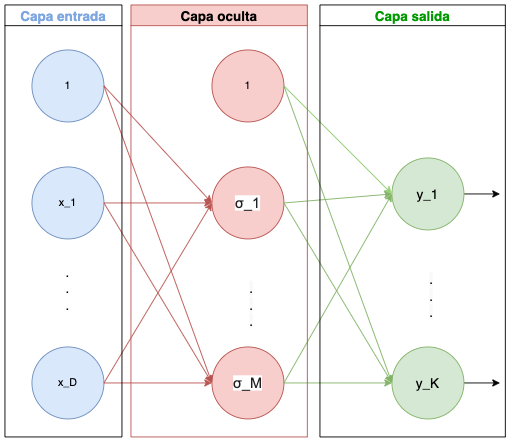
\includegraphics[width=0.65\textwidth]{introduccion_redes_neuronales/construccion_redes_neuronales/red-neuronal-simple-introduccion.drawio.png}
    \caption{Ejemplo de red neuronal con una capa oculta}
    \label{img:ejemplo topología red neuronal}
\end{figure} 
 

En este ejemplo poseemos una capa oculta, 
puede definirse siguiendo esta misma idea
una red neuronal de múltiples capas ocultas. 

% Generalización de modelo 
\subsection{Construcción red neuronal de varias capas ocultas} \label{rrnn:construcción_generalizada}

Etiquetaremos a cada capa con $l \in \{0, \ldots, L \}$, donde $L+1$ es el número total de capas.  Donde 

\begin{itemize}
    \item La capa de entrada será la etiquetada con $l = 0$.
    \item La capa de salida que determina el valor de la red neuronal es la $l=L$.
    \item Las capas ocultas serán aquellas etiquetadas como $0 < l <L.$
\end{itemize}

Se usará un superíndice para hacer referencia a la capa. 
Cada capa posee una dimensión $d^{(l)}$, es decir que posee
$d^{(l)} + 1$ unidades o nodos. El nodo $d_0^{(l)}$ se trata del sesgo y siempre será uno. 

El modelo de red neuronal $\mathcal{H}_{n n}$ viene determinado una vez que se fija la arquitectura de la misma, es decir sus dimensiones $d$. 
\begin{equation}
    d = (d^{(0)}, d^{(1)}, \ldots, d^{(L)})
\end{equation}
y se tiene que cada red neuronal $h \in \mathcal{H}_{n n}$
viene determinada por sus pesos. 

\subsubsection*{Cálculo de una capa oculta}  
Cada nodo recibe una señal de entrada $s$ y determina una salida $x$. 
  
La relación que existe entre dos nodos de capas contiguas es la siguiente: si $x_i^{(l-1)}$ es la salida de la unidad $i$ de la capa $l-1$, 
entonces se calcula la entrada de la unidad $j$ de la capa $l$ como 
\begin{align}\label{eq:construcción_red_neuronas:calculo_una_capa_oculta}
    s_j^{(l)} &= w_{i j}^{(l)} \cdot x_i^{(l-1)}  \\
    x_j^{(l)} &= \theta(s_j^{(l)})
\end{align}

Es decir, que en cada capa $l$ intervienen los siguientes elementos:  
\begin{table}[h]
    \begin{center}
    \begin{tabular}{| l | l | l |}
    \hline
    Elementos & Notación & Representación 
    \\ \hline
    Vector de entrada & $s^{(l)}$ &  Vector de dimensión $d^{(l)}$ \\
    Vector de salida & $x^{(l)}$ &  Vector de dimensión $d^{(l)}+ 1$ \\
    Pesos entrada & $W^{(l)}$ & Matriz de dimensiones $(d^{(l-1)}+1) \times d^{(l)}$ \\
    Pesos salida & $W^{(l+1)}$ 
    & Matriz de dimensiones $(d^{(l)}+1) \times d^{(l+1)}$ \\
    \hline
    \end{tabular}
    \caption{Elementos capa oculta $l$}
    \label{tab:rrnn_elementos_capa_oculta}
    \end{center}
\end{table}

\subsection{ \textit{Forward propagación}}\label{algoritmo-forward-propagation}

Explicaremos en esta sección cómo calcular para una entrada una determinada salida, es decir
dada una red neuronal $h \in \mathcal{H}_{d^{(0)} \times \cdots \times d^{(L)}}$ y un vector de entrada $x \in \mathcal{X}$ calcularemos  $h(x)$, esto se hará gracias al algoritmo conocido como \textit{forward propagation}.

Teniendo presente la relación  explicada en (\refeq{eq:construcción_red_neuronas:calculo_una_capa_oculta}) se puede escribir de forma vectorial la siguiente relación: 
\begin{equation}
    x^{(l)} = 
    \left[ \begin{array}{c}
        1 \\
       \theta(s^{(l)})
        \end{array}
\right] .
\end{equation}
Donde $\theta(s^{(l)})$ es un vector de componentes $\theta(s^{(l)}_j)$. 
Para calcular el vector de entrada de la capa $l$, para cada nodo se hará
\begin{equation}
    s_j^{(l)} = \sum_{i=0}^{d^{(l-1)}} w_{i j}^{(l)}x_i^{(l-1)}.
\end{equation}
Que se formula de forma vectorial para toda la capa como 
\begin{equation}
    s^{(l)} = W^{(l)} x^{(l-1)}.
\end{equation}

Si el vector de entrada es $x \in \mathcal{X} \subseteq \R^d$, 
se inicializa  $x^{(0)} = (1,x_1, \ldots, x_d)^T$ y por tanto $d^{(0)} = d+1.$


La implementación del algoritmo sería:

\begin{algorithm}[H]
    \caption{Algoritmo \textit{Forward propagation} para evaluación de una red neuronal $h_w(x)$.}
    \begin{algorithmic}[1]
        \STATE $x^{(0)} \leftarrow x$ 
        \COMMENT{Inicialización}

        \STATE \COMMENT{\textit{Forward Propagation}}
        \For{$l = 1, \ldots , L$}{
            % Calcula s
            \STATE 
            \begin{equation}
                s^{(l)}
                    \leftarrow
                    \left(W^{(l)}\right)^T
                    x^{(l-1)}      
            \end{equation}

            %Calcula x
            \STATE
            \begin{equation}
                x^{(l)}
                    \leftarrow
                    \left[ 
                        \begin{array}{c}
                            1 \\ 
                            \theta \left( s^{(l)}\right)
                        \end{array}
                    \right]
            \end{equation}
        }
        \STATE $h_w(x) = x^{(L)}$ 
        \COMMENT{Salida}  
\end{algorithmic}
\end{algorithm}

% Imagen red neuronal con pesos concretos
Veamos un ejemplo concreto para la siguiente red neuronal de la imagen \ref{img:construccion_rrnn:rrnn-2-3-2-1}
\begin{figure}[h!]
    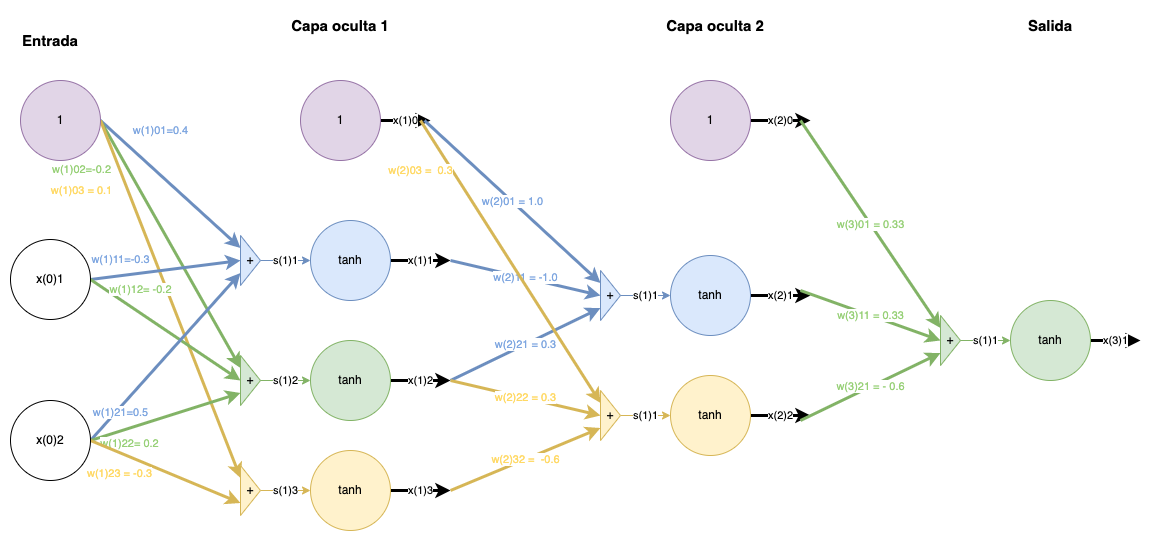
\includegraphics[width=\textwidth]{introduccion_redes_neuronales/construccion_redes_neuronales/rrnn-2-3-2-1-completa.png}
    \caption{Ejemplo de red neuronal con dos capas ocultas y pesos con valores concretos}
    \label{img:construccion_rrnn:rrnn-2-3-2-1}
\end{figure} 

La red de la imagen \ref{img:construccion_rrnn:rrnn-2-3-2-1} está 
compuesta por dos capas ocultas, acepta vectores de entrada de dimensión dos, 
la primera capa oculta está compuesta por tres neuronas, 
la segunda por dos y la salida por una. 
La notación del dibujo usada es la siguiente, entre paréntesis se 
especifica la capa, en el caso de la salida $x(l)i$ hace referencia a la salida $i$-ésima de la capa $l$. Las \textit{flechas} que conectan los nodos $w(l)ij$ hace referencia al peso que se le da a $x(l-1)i$ con respecto a la entrada $s(l)j$.

Representando los pesos de manera matricial
\begin{align}
    W^{(l)} = 
    \begin{bmatrix}
        w^{(l)}_{01} & w^{(l)}_{11} & \cdots & w^{(l)}_{d^{(l-1)} 1}\\
        w^{(l)}_{02} & w^{(l)}_{12} & \cdots & w^{(l)}_{d^{(l-1)} 2}\\
        \cdots & \cdots & \cdots & \cdots \\
        w^{(l)}_{0d} & w^{(l)}_{1d} & \cdots & w^{(l)}_{d^{(l-1)} d}\
    \end{bmatrix} 
\end{align}
las matrices de pesos de nuestra imagen son :
\begin{align}
    W^{(1)} = 
    \begin{bmatrix}
        0.4 & -0.3 & 0.5\\
        -0.2 & -0.2 & 0.2\\
        0.1 & 0 & -0.3
    \end{bmatrix} ,
    W^{(2)} = 
    \begin{bmatrix}
        1 & -1 & 0.3 & 0\\
        0.3& 0 & 0.3 & -0.6 
    \end{bmatrix} ,
    W^{(3)} = 
    \begin{bmatrix}
        0.33 & 0.33 & -0.6 \
    \end{bmatrix} .
\end{align}
Si inicializamos $x= (1,0)$ y tomamos como función de activación
a la tangente hiperbólica, la ejecución del algoritmo queda reflejada en la tabla \ref{tab:construcción_rnnn:ejemplo_forward_propagation} resultando que 
$h((1,0)) = 0.439$.
\begin{table}[H]
    \begin{center}
\begin{tabular}{| c | c | c | c| }
    \hline
    Capa $l$-ésima &  $W^{(l)}$ & $\bigl(s^{(l)}\bigr)^T $ & $\bigl(x^{(l)}\bigr)^T$ \\ \hline
    0 & & & $(1,1,0)$ 
    \\ \hline
    1 & 
    $\begin{bmatrix}
        0.4 & -0.3 & 0.5\\
        -0.2 & -0.2 & 0.2\\
        0.1 & 0 & -0.3
    \end{bmatrix}$ 
    & $(0.1, -0.4, 0.1)$ & $(1, 0.1, -0.38, 0.1)$
     \\ \hline
    2 & $\begin{bmatrix}
        1 & -1 & 0.3 & 0\\
        0.3& 0 & 0.3 & -0.6 
    \end{bmatrix}$
    & $(0.786, 0.126)$
    & $(1,0.656, 0.126)$
    \\ \hline
    3 & $\begin{bmatrix}
        0.33 & 0.33 & -0.6 
    \end{bmatrix}$ 
    & $(0.471)$ 
    & $(1,0.439)$
    \\ \hline
\end{tabular}
\caption{Ejemplo de ejecución del algoritmo de \textit{forward propagation}}
\label{tab:construcción_rnnn:ejemplo_forward_propagation}
\end{center}
\end{table}
